\documentclass{../Vorlage/mat}
\usepackage{upgreek}
\usetikzlibrary{shapes.misc}
\lstset{
	basicstyle=\small
}

\begin{document}
\maketitle{Sebastian Bliefert}{}{Nils Drebing}{}{Pascal Pieper}{}{25.01.2017}{4} \\

\section*{1. Theorie zu Filtermethoden}
\subsection*{Wahrscheinlichkeitsdichtefunktion}
Die Gaussglockenkurve ist wie folgt definiert:
\begin{equation}
	\upvarphi(x, \sigma, \mu) = \dfrac{1}{\sigma\sqrt{2\pi}}e^{-\frac{1}{2}\left(\dfrac{x-\mu}{\sigma}\right)^2}
\end{equation}

Das Integral jeder Wahrscheinlichkeitsfunktion ergibt immer 1. Das
 ist gleichbedeutend mit der Aussage, dass $P(\Omega) = 1$, also die Wahrscheinlichkeit, dass \textit{irgend ein} Ergebnis stattfindet, ist sicher.

\subsection*{Abhängigkeit von Wahrscheinlichkeiten}

Die Abhängigkeit zweier Zufallsvariablen bezeichnet man durch deren Covarianz, also $Cov(x,y) \neq 0$. Ferner sind zwei Zufallsvariablen genau dann unabhängig, wenn $P_{XY}(x_i;y_j) = P_X(x_i)\cdot P_Y(y_j)$ gilt. Daraus folgt, dass sie dann unabhängig sind , wenn $P(x) = P(x | y)$ und $P(y) = P(y | x)$ gilt.

a) 
$P(A) = 0.5 , P(B) = 0.25, P(A|B) = 1$, also abhängig.\\
b)
$P(A) = 0.5, P(B) = \frac{1}{16}, P(A|B) = 0$, also abhängig.\\
c)
$P(A) = 0.5, P(B) = 0.5, P(A|B) = P(B|A) = 0.5$, also unabhängig.


\subsection*{Bayes-Theorem}
Das Theorem beschreibt, dass die Wahrscheinlichkeit für ein Ereignis A unter der Annahme, dass ein anderes Ereignis B eingetreten ist, gleich der Wahrscheinlichkeit des Eintretens von B unter der Annahme von A multipliziert mit der reinen Wahrscheinlichkeit von A geteilt durch der reinen Wahrscheinlichkeit von B ist.

$P(B) = \frac{11}{20}, P(W) = \frac{9}{20}, P(L) = \frac{13}{20}, P(R) = \frac{7}{20}$\\
$P(W|L) = \frac{6}{13}, P(B|L) = \frac{7}{13}, P(W|R) = \frac{3}{7}, P(B|R) = \frac{4}{7}$\\
$P(L|W) = \frac{2}{3}, P(R|W) = \frac{3}{9}, P(L|B) = \frac{7}{11}, P(R|B) = \frac{4}{11}$\\
\\
$P(L|W) = \dfrac{P(W|L) \cdot P(L)}{P(R)} = \dfrac{\frac{6}{13} \cdot \frac{13}{20}}{\frac{9}{20}} = \frac{2}{3}$\\
$P(W|L) = \dfrac{P(L|W) \cdot P(W)}{P(L)} = \dfrac{\frac{2}{3} \cdot \frac{9}{20}}{\frac{13}{20}} = \frac{6}{13}$


\section*{2. Partikelfilter zur Rollstuhllokalisation}
\subsection*{Fehlerhafte Konvergenz}
Grundsätzlich wäre es möglich, dass ein Partikelfilter zu einer falschen Position konvergiert.\\
Nehmen wir eine hypothetische Karte mit zwei absolut gleich beschaffenen Sektoren an. Der Partikelfilter stellt in beiden Sektoren eine Position mit hoher Wahrscheinlichkeit fest. Durch Zufall wird jedoch beim Ziehen aus dem temporären Partikelset die reale Position nicht gezogen, sondern nur ihr Pendant im anderen Sektor. Ab diesem Moment würde der Partikelfilter möglicherweise zur Position im falschen Sektor konvergieren. Dieses Szenario ist allerdings sehr konstruiert und somit entsprechend unwahrscheinlich.\\
Im Normalfall sollte der Partikelfilter zur richtigen Position konvergieren, da auch bei sehr ähnlichen Positionen irgendwann ein entscheidender Unterschied in Erscheinung tritt, durch den die falsche Position sehr unwahrscheinlich wird und somit die richtige Position als einzige wahrscheinliche verbleibt.
\subsection*{Bestimmung des Zustandsvektors}
Der Zustand des Rollstuhls sollte in diesem Szenario mindestens durch eine X,Y Position und eine Rotation beschrieben werden. Zusätzlich könnte noch eine Z Position und evtl. durch roll und neigungswinkel beschrieben werden. Letztere sind allerdings für die Lösung der Aufgabe nicht unbedingt relevant.
\subsection*{Bestimmung des Messvektors}
Der Messvektor beinhaltet die von den Laserscannern gemessenen Entfernungen. Praktisch wären hier noch Informationen aus einer IMU, um die Partikel zuverlässiger samplen zu können.
\subsection*{Schritte der Filterung mit einem Partikelfilter}
Der Algorithmus des Partikelfilters kann grob in zwei Teile aufgeteilt werden.
\subsubsection*{1. Generierung des temporären Partikelsets}
\begin{enumerate}
	\item Es wird für jeden im Partikelset des vorherigen Durchlaufes enthaltenen Partikel ein neues Partikel gesamplet. Dies geschieht jeweils auf Basis des entsprechenden Partikels aus dem vorherigen Set. Dabei wird etwas Rauschen mit eingefügt, damit identische Partikel trotzdem leicht unterschiedlich neu gesamplet werden.
	\item Für den jeden neu gesampleten Partikel wird die Wahrscheinlichkeit, dass er dem Realzustand entspricht berechnet. Dafür wird ein Messvektor für diesen Partikel simuliert und mit dem tatsächlichen Messvektor verglichen. Diese Wahrscheinlichkeit wird im folgenden Schritt als das Gewicht bezeichnet.
	\item Die neu gesampleten Partikel werden in das temporäre Partikelset eingetragen.
\end{enumerate}
\subsubsection*{2. Generierung des eigentlichen Partikelsets}
Der folgende Vorgang wird so oft ausgeführt, wie es Partikel im temporären Partikelset gibt.
\begin{enumerate} 
	\item Unter Berücksichtigung des Gewichtes der einzelnen Partikel wird ein Partikel aus dem temporären Partikelset gezogen (mit Zurücklegen). Die Wahrscheinlichkeit, dass ein spezifischer Partikel gezogen wird, ist dabei proportional zu seinem Gewicht.
	\item Der gezogene Partikel wird nun zum eigentlichen Partikelset hinzugefügt.
\end{enumerate}
Das resultierende Partikelset enthält am Ende dieses Abschnittes genau so viele Partikel wie das temporäre Partikelset und somit auch genau so viele wie das aus dem vorherigen Durchgang. Weiterhin können (und sollen sogar) Partikel mehrfach enthalten sein, was wichtig für die Konvergenz zur richtigen Position ist.
\subsubsection*{Übergabeparameter}
Dem Partikelfilter müssen das Partikelset aus dem vorherigen Durchgang, der Messvektor und die Steuerungsinformationen seit dem letzten Durchgang übergeben werden.\\

\section*{3. Implementierung der Lokalisation mit einem Partikelfilter}
\subsection*{Quellcode}
\lstset{language=python}
Die Implemengtierung des Partikelfilters erfolgt in der \textit{behaviour.py}. Um das Datenmanagement zu vereinfachen, wurde eine Klasse \textit{State} entworfen. Diese speichert die benötigten Werte wie Koordinaten, Rotation und Gewicht eines Partikels.
\begin{lstlisting}
# class handling particles and weights
class State:
    x = 0.
    y = 0.
    z = 0.
    rot = 0.
    weight = 0.

    def __init__(self,x,y,z,rot, weight):
        self.x = x
        self.y = y
        self.z = z
        self.rot = rot
        self.weight = weight
\end{lstlisting}

Die Partikel werden stets zufällig initialisiert.

\begin{lstlisting}
#initializes particles as states
def initParticles():
    magicDistances = 7 # set points on map
    global particles
    data = pointCloudData["particles"]
    for i in range(getNumberOfParticles()):
        # randomly initialize particles
        part = State(random.uniform(-magicDistances,magicDistances),
                         random.uniform(-magicDistances,magicDistances),
                         0., 
                         random.uniform(-np.pi, np.pi), 1./getNumberOfParticles())
        particles.append(part)
    particles[0] = State(0,0,0,0,1./getNumberOfParticles())
\end{lstlisting}

Das Bewegungsmodell wird direkt im der Sampling-Methode der Partikel implementiert. Hier wird der gegebene Controlinput in $\frac{m / s}{rad}$ umgerechnet. Die Noisefaktoren wurden dabei experimentell ermittelt. Bei stärkerer Beschleunigung soll das Rauschen auch entsprechend stärker sein.

\begin{lstlisting}
#samples particle. takes particle to update and control input
def sampleParticle(particle, control):
    global particles
    ##### BEWEGUNGSMODELL #####
    #calculates velocitys based on the control input
    megaMagicNoiseFactor = 5 + 0 * (1 - particle.weight)
    noiseFactorl = 1 + abs(control[0] * megaMagicNoiseFactor)
    noiseFactorr = 1 + abs(control[1] * megaMagicNoiseFactor)
    left = control[0]
    right = control[1]
    if(noiseFactorl > 0):
        left = np.random.normal(control[0], noiseFactorl)
    if(noiseFactorr > 0):
        right = np.random.normal(control[1], noiseFactorr)
    updateTime = 0.0175
    diam = 0.3
    width= 0.54
    circ = diam * np.pi
    rang = [left / (2 * np.pi * circ) * updateTime, right / (2 * np.pi * circ) * updateTime]

    dist = (rang[0] + rang[1])/2
    angle = (rang[1] - rang[0]) / float(width)
    particle.x += dist * math.cos(particle.rot)
    particle.y += dist * math.sin(particle.rot)
    particle.rot += angle
    particle.rot %= (2 * np.pi)
    if particle.rot < -np.pi:
        particle.rot += 2 * np.pi
    elif particle.rot > np.pi:
        particle.rot -= 2*np.pi

    return particle
\end{lstlisting}

Das Messmodell wird in der \textit{probMeasurement}-Methode verwendet. Als Eingaben werden hier Position und Rotation erwartet. Als Fehlermaß zwischen dem gemessenen und hypothetischen Zustand dient der quadratische Fehler der Laserscanns.

\begin{lstlisting}
## returns measurement on a given position with the given orientation
def probMeasurement(position, rotation):
    global laserRange
    #### PERCEPTION MODEL###
    # Laser scanner positions fl, fr, bl, br
    basePos = np.array([[ 0.320234,  0.230233],
                        [ 0.320234, -0.230234],
                        [-0.306395,  0.214315],
                        [-0.306395, -0.214316]])

    baseRotz = np.array([0.785, 3*0.785, -0.785, -3*0.785])
    directions = np.array([0.262, -1.309, 1.833, -2.879])
    magicWinkel_offset = 0.349
    laserWinkelOffsets = np.array([magicWinkel_offset / 2 + magicWinkel_offset,
                            magicWinkel_offset / 2, -magicWinkel_offset/2,
                            -(magicWinkel_offset/2+magicWinkel_offset)])

    basePos = [rot2d(bp, -rotation) for bp in basePos]
    basePos = [np.array(bp) + np.array([position[0], position[1]]) for bp in basePos]

    laser = np.array([0, laserRange])
    targetpoint = [np.array(rot2d(laser, i - rotation)) for i in baseRotz]  #45fucks
    multiLaserTargetPoints = []
    for elem in targetpoint:
        multiLaserTargetPoints.append([np.array(rot2d(elem, offs)) for offs in laserWinkelOffsets])

    multiLaserTargetPointsTranse = []
    for  i in range(len(basePos)):
        multiLaserTargetPointsTranse.append([sub+basePos[i] for sub in multiLaserTargetPoints[i]])

    calced = []
    for i in range(len(multiLaserTargetPointsTranse)):
        for j in range(len(multiLaserTargetPointsTranse[i])):
            dist = checkDistance(basePos[i], multiLaserTargetPointsTranse[i][j])
            if dist > 1:
                calced.append(laserRange)
            else:
                calced.append(dist * laserRange)
    return calced

## calculates the probability of a particle. Uses squared error
def calcProb(list1, list2):
    global laserRange
    err2 = sum((np.array(list1) - np.array(list2))**2)
    return (1 - err2 / ((laserRange**2)*len(list1)))
\end{lstlisting}

Der Algorithmus des Partikelfilters erhält als Eingaben die Menge der Partikel, die Joystickeingabe und die Messungen der Laserscanner im Roboterkoordinatensystem.

\begin{lstlisting}
def particleFilter(particles, control, measurement):
    newParticles = []
    resultParticles = []
    for i in range(len(particles)):
        p = sampleParticle(particles[i], control)
        p.weight = calcProb(probMeasurement((p.x,p.y),p.rot),measurement) * p.weight
        newParticles.append(p)
    weightSum = 0.
    weightMax = 0.
    for p in newParticles:
        if(p.weight > weightMax):
            weightMax = p.weight
        weightSum += p.weight

 p.weight))
    for i in range(getNumberOfParticles()):
        rnd = np.random.uniform(0, weightSum)
        ws = 0
        for p in newParticles:
            ws += p.weight
            if ws >= rnd:
                resultParticle = State(p.x, p.y, p.z, p.rot, p.weight)
                resultParticle.weight /= weightMax
                resultParticles.append(resultParticle)
                break

    return resultParticles
\end{lstlisting}

Als approximierte Position wird das Mittel der x- und y-Werte ausgegeben.
\newpage
\subsection*{Experimente}
Für die Experimente wurde die Schritt-ausführen-Funktion der MARS-Umgebung verwendet. Als initiale Rotationen und Position erhielt jedes Partikel stets randomisierte, normalverteite Werte.

\subsubsection*{150 Partikel}
\begin{figure}[!htbp]
\centering
\begin{minipage}{.5\textwidth}
  \centering
  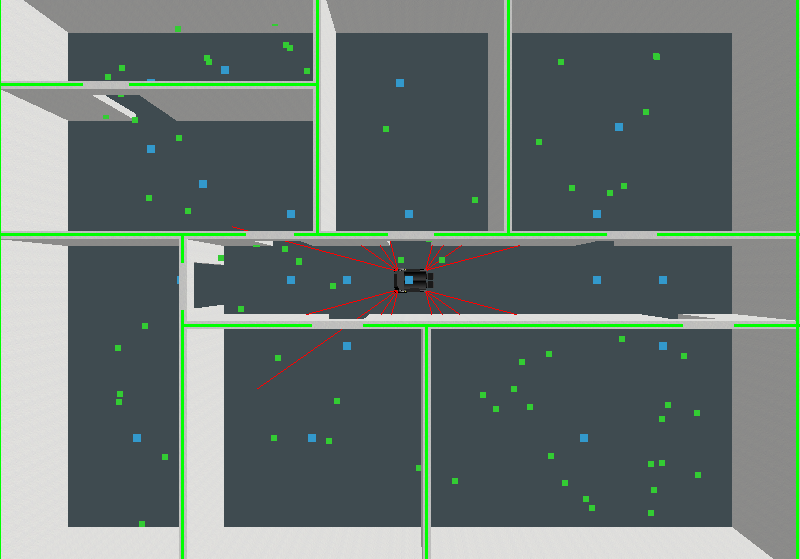
\includegraphics[scale=0.25]{1_150_schlecht.png}
  \captionof{figure}{Verteilung nach 1. Zug. Grüne Punkte sind die Partikel.}
  \label{fig1}
\end{minipage}%%
\begin{minipage}{.5\textwidth}
  \centering
  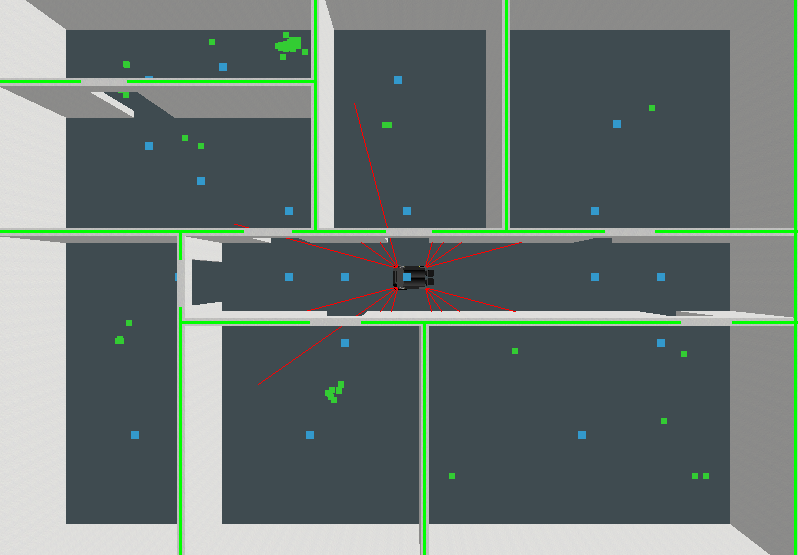
\includegraphics[scale=0.25]{1_150_schlecht_nach_6.png}
  \captionof{figure}{Verteilung nach 6. Zug. Punktemenge clustert sich im Nordwesten}
  \label{fig2}
\end{minipage}
\centering
\begin{minipage}{.5\textwidth}
  \centering
  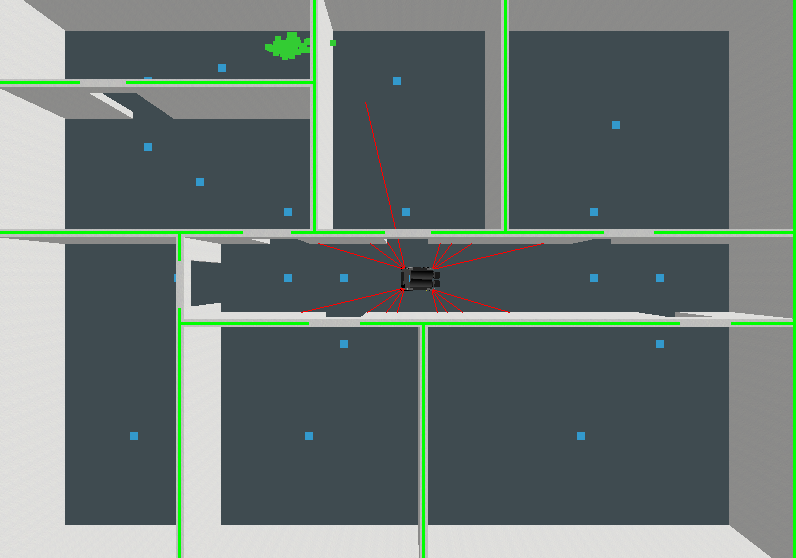
\includegraphics[scale=0.25]{1_150_schlecht_nach_13.png}
  \captionof{figure}{Nach 13 Kalkulationen fehlerhaft im Nordwesten approximiert}
  \label{fig3}
\end{minipage}%%
\begin{minipage}{.5\textwidth}
\end{minipage}
\end{figure}

Unter der Verwendung von lediglich 150 Partikeln konvergiert der Algorithmus nur in seltenen Fällen korrekt. Zum einen spielt die initiale Partikelverteilung dabei eine wichtige Rolle. Zum anderen ähneln sich einige Räume in Bezug auf ihr Layout. Somit kommen auch andere Räume für die Messungen des Flurs in Frage.
\newpage
\subsubsection*{500 Partikel}
\begin{figure}[!htbp]
\centering
\begin{minipage}{.5\textwidth}
  \centering
  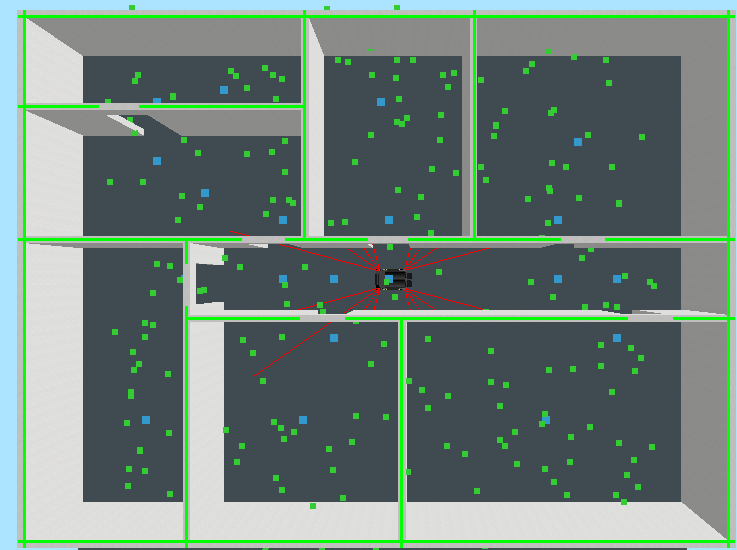
\includegraphics[scale=0.25]{1_500_gut.png}
  \captionof{figure}{Verteilung nach 1. Zug. Grüne Punkte sind die Partikel.}
  \label{fig4}
\end{minipage}%%
\begin{minipage}{.5\textwidth}
  \centering
  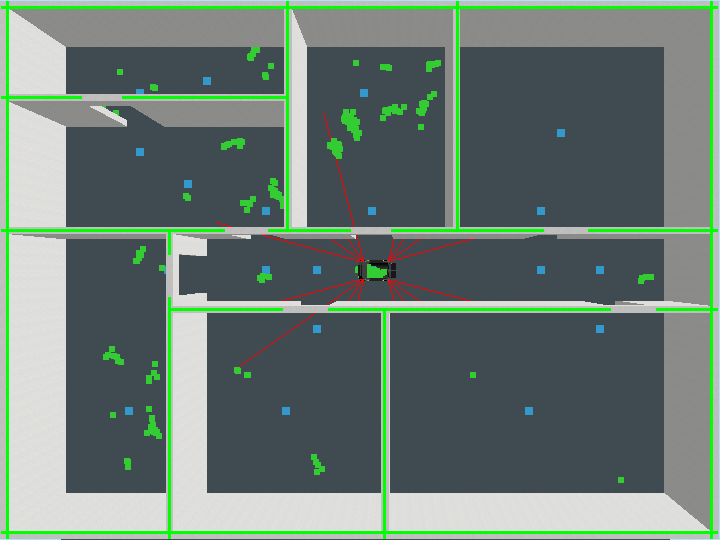
\includegraphics[scale=0.25]{1_500_nach_4.png}
  \captionof{figure}{Verteilung nach 4 Schritten. Punktemenge clustert sich an mehreren Stellen, einschließlich der Rollstuhlposition}
  \label{fig5}
\end{minipage}
\centering
\begin{minipage}{.5\textwidth}
  \centering
  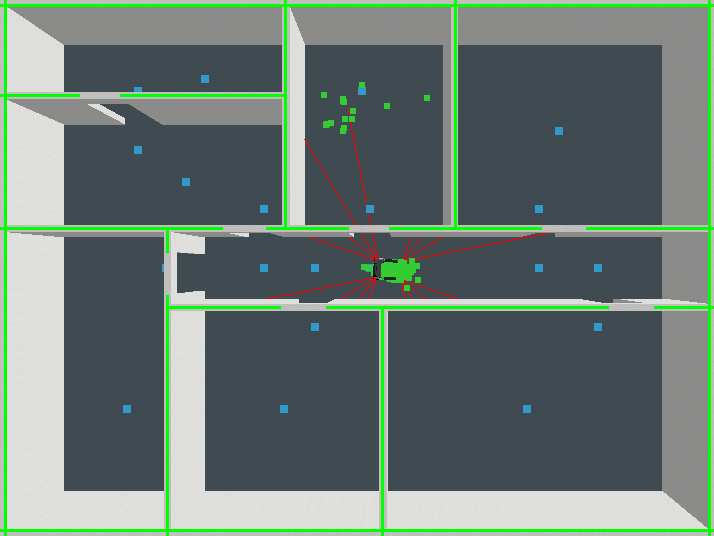
\includegraphics[scale=0.25]{1_500_gut_nach_18.png}
  \captionof{figure}{Verteilung nach 18 Schritten. Algorithmus konvergiert in der Nähe des Verhikels}
  \label{fig6}
\end{minipage}%%
\begin{minipage}{.5\textwidth}
  \centering
  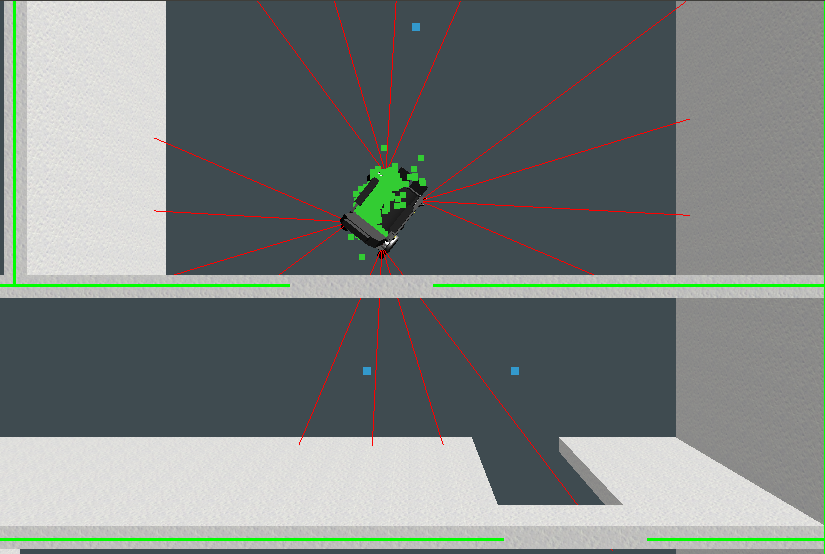
\includegraphics[scale=0.25]{1_500_gut_in_fahrt.png}
  \captionof{figure}{Verteilung während der Fahrt mit einer kurvigen Trajektorie. Geschwindigkeit: $10 \frac{rad}{s}$}
  \label{fig7}
\end{minipage}
\begin{minipage}{.5\textwidth}
  \centering
  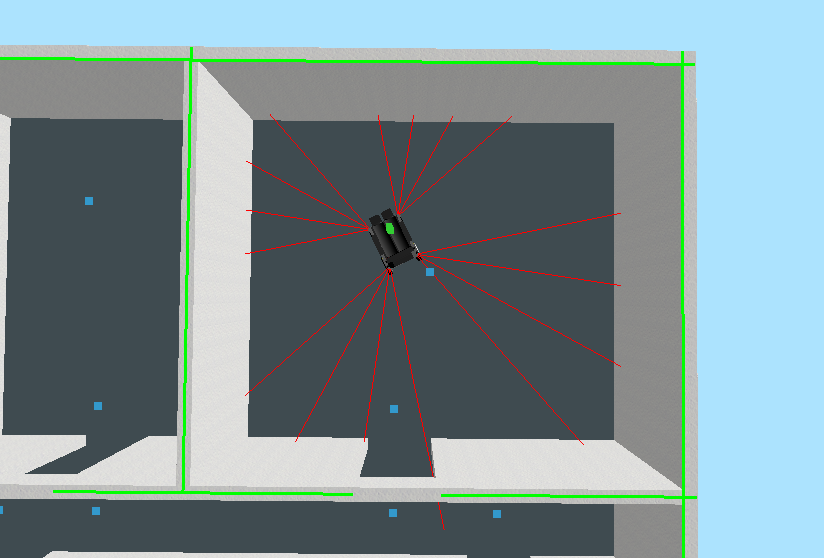
\includegraphics[scale=0.25]{1_500_gut_konvergiert.png}
  \captionof{figure}{Verteilung, nachdem das Verhikel keine Eingaben über einen kurzen Zeitraum bekommt.}
  \label{fig8}
\end{minipage}
\end{figure}

Werden 500 Partikel in dem Algorithmus verwendet, so wird der Rollstuhl deutlich häufiger lokalisiert. Dies ist zum einen damit zu begründen, dass eine größere Menge an Partikeln initial in der Nähe des Rollstuhls landen und damit der tatsächlichen Messungen ähneln.\\
Während der Fahrt verteilen sich die Partikel, gegeben des implementierten Messrauschen, sinnvoll um das Vehikel (Abbildung \ref{fig7}). Somit sind sowohl Mess- als auch Bewegungsmodell präzise genug. Steht der Rollstuhl über mehrere Zyklen, so konvergieren die Partikel in Richtung einer expliziten Position (Abbildung \ref{fig8}).
\newpage
\subsubsection*{Rotation an der Wand}
\begin{figure}[!htbp]
  \centering
  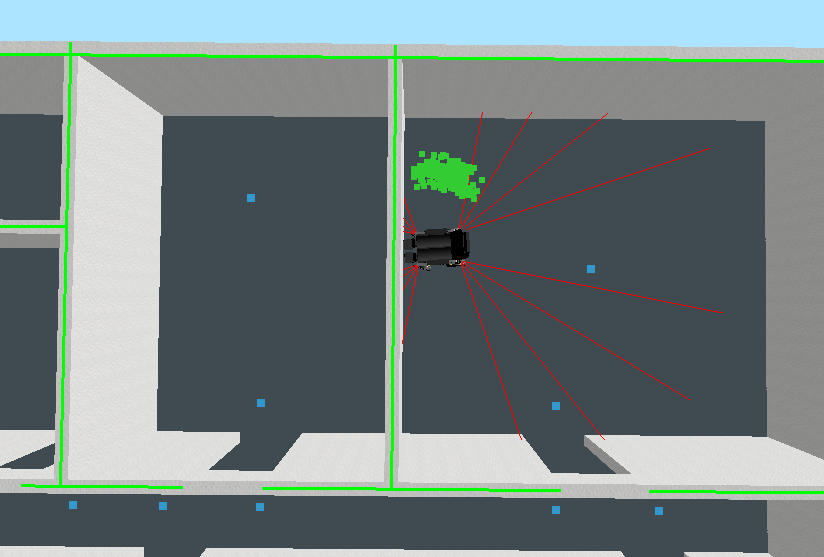
\includegraphics[scale=0.3]{1_500_fehler_rotation.png}
  \captionof{figure}{Fehlerfall: Beim Manövieren an einer Wand verschiebt sich die Verteilung}
  \label{fig9}
\end{figure}

Wird das Vehikel gegen eine Wand manövriert und anschließend weiter Kontrolleingaben in Richtung dieser Wand getätigt, so verschiebt sich die Verteilung (siehe Abbildung \ref{fig9}). Dies ist damit zu begründen, dass das Bewegungsmodell nicht für den Fall konzipiert wurde ist, dass sich die Position und Rotation bei Joystickeingaben nicht verändern.
>>>>>>> Stashed changes
>>>>>>> Stashed changes
\end{document}
